\section{Project Framing and Strategic Context}

\subsection{Executive Overview}

This project aims to establish a \textbf{world-class immersive visualisation facility} – a next-generation CAVE (Cave Automatic Virtual Environment) that will serve as a national academic platform for research in automation, robotics, risk management, nuclear engineering, advanced manufacturing, and beyond. The system will enable teams of researchers (up to 6 simultaneously) to step inside shared, life-size 3D simulations without wearing VR headsets, fostering unprecedented collaborative research capabilities.

\begin{figure}[h]
\centering
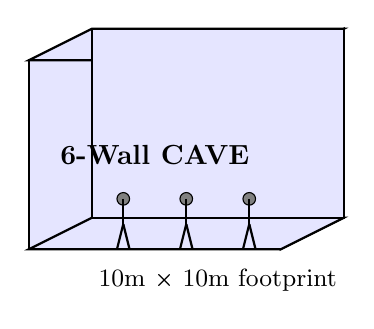
\begin{tikzpicture}[scale=0.8]
    % Draw 6-wall CAVE
    \draw[thick, fill=blue!10] (0,0) rectangle (4,3);
    \draw[thick, fill=blue!10] (4,0) -- (5,0.5) -- (5,3.5) -- (4,3) -- cycle;
    \draw[thick, fill=blue!10] (0,3) -- (1,3.5) -- (5,3.5) -- (4,3) -- cycle;
    \draw[thick, fill=blue!10] (0,0) -- (1,0.5) -- (5,0.5) -- (4,0) -- cycle;
    \draw[thick, fill=blue!10] (1,0.5) -- (1,3.5) -- (5,3.5) -- (5,0.5) -- cycle;
    
    % Add labels
    \node at (2,1.5) {\textbf{6-Wall CAVE}};
    \node at (3,-0.5) {\small 10m × 10m footprint};
    
    % Add people silhouettes
    \foreach \x in {1.5,2.5,3.5} {
        \draw[fill=gray] (\x,0.8) circle (0.1);
        \draw[thick] (\x,0.8) -- (\x,0.4);
        \draw[thick] (\x,0.4) -- (\x-0.1,0);
        \draw[thick] (\x,0.4) -- (\x+0.1,0);
    }
\end{tikzpicture}
\caption{Conceptual view of the 6-wall immersive facility with multi-user capability}
\end{figure}

\subsection{Strategic Value Proposition}

The facility will deliver transformative value across multiple dimensions:

\begin{itemize}
    \item \textbf{Research Excellence}: Enable breakthrough research through unprecedented visualisation capabilities
    \item \textbf{Industry Partnerships}: Attract commercial collaborations worth £500k+ annually
    \item \textbf{Talent Attraction}: Draw world-class researchers and students to the institution
    \item \textbf{National Infrastructure}: Position the UK at the forefront of immersive technology research
\end{itemize}

\subsection{Key Technical Specifications}

\begin{table}[h]
\centering
\begin{tabular}{|l|l|}
\hline
\textbf{Parameter} & \textbf{Specification} \\
\hline
Configuration & 6-sided immersive space (4 walls + floor + ceiling) \\
\hline
Physical Dimensions & 25m × 20m footprint, double-height (6-7m) \\
\hline
Display Resolution & 8K per surface (minimum 4K native) \\
\hline
Multi-user Support & Up to 6 concurrent users with stereoscopic 3D \\
\hline
Frame Rate & 120+ Hz per eye (240-360 Hz total for multi-user) \\
\hline
Tracking Accuracy & Sub-millimetre precision optical tracking \\
\hline
Audio System & Wave Field Synthesis with 128-512 speakers \\
\hline
Compute Backend & 32+ high-end GPUs in clustered configuration \\
\hline
Volumetric Capture & 32-64 camera array for real-time 3D reconstruction \\
\hline
\end{tabular}
\caption{Core technical specifications for the world-class immersive facility}
\end{table}

\subsection{Investment Scale and Timeline}

The estimated capital investment for this world-class facility is in the order of \textbf{several million pounds}, reflecting our ambition to create one of the most advanced installations globally. The project timeline spans approximately 24 months from initiation to operational status.

\begin{figure}[h]
\centering
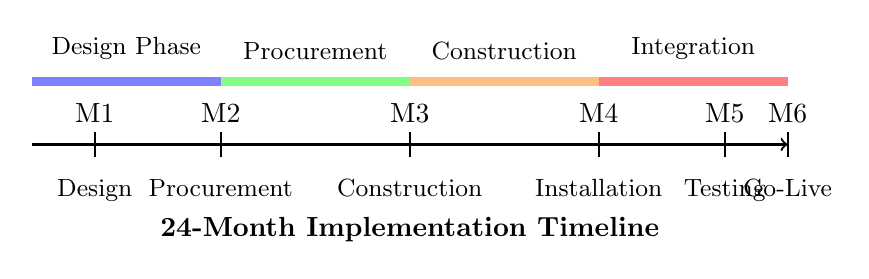
\begin{tikzpicture}[scale=0.8]
    % Timeline
    \draw[thick, ->] (0,0) -- (12,0);
    
    % Milestones
    \foreach \x/\label/\desc in {1/M1/Design, 3/M2/Procurement, 6/M3/Construction, 9/M4/Installation, 11/M5/Testing, 12/M6/Go-Live} {
        \draw[thick] (\x,0) -- (\x,0.2);
        \draw[thick] (\x,0) -- (\x,-0.2);
        \node[above] at (\x,0.2) {\label};
        \node[below, font=\small] at (\x,-0.4) {\desc};
    }
    
    % Phases
    \draw[thick, blue!50, line width=3pt] (0,1) -- (3,1);
    \draw[thick, green!50, line width=3pt] (3,1) -- (6,1);
    \draw[thick, orange!50, line width=3pt] (6,1) -- (9,1);
    \draw[thick, red!50, line width=3pt] (9,1) -- (12,1);
    
    \node[above] at (1.5,1.2) {\small Design Phase};
    \node[above] at (4.5,1.2) {\small Procurement};
    \node[above] at (7.5,1.2) {\small Construction};
    \node[above] at (10.5,1.2) {\small Integration};
    
    \node[below] at (6,-1) {\textbf{24-Month Implementation Timeline}};
\end{tikzpicture}
\caption{High-level project timeline showing major phases and milestones}
\end{figure}

\subsection{Stakeholder Landscape}

The project's success depends on effective engagement with multiple stakeholder groups:

\begin{enumerate}
    \item \textbf{University Leadership}: Strategic alignment and funding approval
    \item \textbf{Research Community}: Primary users spanning multiple faculties
    \item \textbf{Industry Partners}: Nuclear, automotive, aerospace, and manufacturing sectors
    \item \textbf{Government Bodies}: UK Research Councils and innovation agencies
    \item \textbf{Technology Vendors}: Digital Projection, NVIDIA, tracking system providers
\end{enumerate}

\subsection{Alignment with National Priorities}

This facility directly supports key UK strategic initiatives:

\begin{itemize}
    \item \textbf{Industrial Strategy}: Advancing Industry 4.0 and digital manufacturing
    \item \textbf{Nuclear Sector Deal}: Enabling safe decommissioning through virtual training
    \item \textbf{Autonomous Systems}: Supporting CAV development and testing
    \item \textbf{Net Zero Goals}: Optimising industrial processes through simulation
\end{itemize}